% Options for packages loaded elsewhere
\PassOptionsToPackage{unicode}{hyperref}
\PassOptionsToPackage{hyphens}{url}
\PassOptionsToPackage{dvipsnames,svgnames,x11names}{xcolor}
%
\documentclass[
]{article}
\usepackage{amsmath,amssymb}
\usepackage{iftex}
\ifPDFTeX
  \usepackage[T1]{fontenc}
  \usepackage[utf8]{inputenc}
  \usepackage{textcomp} % provide euro and other symbols
\else % if luatex or xetex
  \usepackage{unicode-math} % this also loads fontspec
  \defaultfontfeatures{Scale=MatchLowercase}
  \defaultfontfeatures[\rmfamily]{Ligatures=TeX,Scale=1}
\fi
\usepackage{lmodern}
\ifPDFTeX\else
  % xetex/luatex font selection
\fi
% Use upquote if available, for straight quotes in verbatim environments
\IfFileExists{upquote.sty}{\usepackage{upquote}}{}
\IfFileExists{microtype.sty}{% use microtype if available
  \usepackage[]{microtype}
  \UseMicrotypeSet[protrusion]{basicmath} % disable protrusion for tt fonts
}{}
\makeatletter
\@ifundefined{KOMAClassName}{% if non-KOMA class
  \IfFileExists{parskip.sty}{%
    \usepackage{parskip}
  }{% else
    \setlength{\parindent}{0pt}
    \setlength{\parskip}{6pt plus 2pt minus 1pt}}
}{% if KOMA class
  \KOMAoptions{parskip=half}}
\makeatother
\usepackage{xcolor}
\usepackage[margin=1in]{geometry}
\usepackage{color}
\usepackage{fancyvrb}
\newcommand{\VerbBar}{|}
\newcommand{\VERB}{\Verb[commandchars=\\\{\}]}
\DefineVerbatimEnvironment{Highlighting}{Verbatim}{commandchars=\\\{\}}
% Add ',fontsize=\small' for more characters per line
\usepackage{framed}
\definecolor{shadecolor}{RGB}{248,248,248}
\newenvironment{Shaded}{\begin{snugshade}}{\end{snugshade}}
\newcommand{\AlertTok}[1]{\textcolor[rgb]{0.94,0.16,0.16}{#1}}
\newcommand{\AnnotationTok}[1]{\textcolor[rgb]{0.56,0.35,0.01}{\textbf{\textit{#1}}}}
\newcommand{\AttributeTok}[1]{\textcolor[rgb]{0.13,0.29,0.53}{#1}}
\newcommand{\BaseNTok}[1]{\textcolor[rgb]{0.00,0.00,0.81}{#1}}
\newcommand{\BuiltInTok}[1]{#1}
\newcommand{\CharTok}[1]{\textcolor[rgb]{0.31,0.60,0.02}{#1}}
\newcommand{\CommentTok}[1]{\textcolor[rgb]{0.56,0.35,0.01}{\textit{#1}}}
\newcommand{\CommentVarTok}[1]{\textcolor[rgb]{0.56,0.35,0.01}{\textbf{\textit{#1}}}}
\newcommand{\ConstantTok}[1]{\textcolor[rgb]{0.56,0.35,0.01}{#1}}
\newcommand{\ControlFlowTok}[1]{\textcolor[rgb]{0.13,0.29,0.53}{\textbf{#1}}}
\newcommand{\DataTypeTok}[1]{\textcolor[rgb]{0.13,0.29,0.53}{#1}}
\newcommand{\DecValTok}[1]{\textcolor[rgb]{0.00,0.00,0.81}{#1}}
\newcommand{\DocumentationTok}[1]{\textcolor[rgb]{0.56,0.35,0.01}{\textbf{\textit{#1}}}}
\newcommand{\ErrorTok}[1]{\textcolor[rgb]{0.64,0.00,0.00}{\textbf{#1}}}
\newcommand{\ExtensionTok}[1]{#1}
\newcommand{\FloatTok}[1]{\textcolor[rgb]{0.00,0.00,0.81}{#1}}
\newcommand{\FunctionTok}[1]{\textcolor[rgb]{0.13,0.29,0.53}{\textbf{#1}}}
\newcommand{\ImportTok}[1]{#1}
\newcommand{\InformationTok}[1]{\textcolor[rgb]{0.56,0.35,0.01}{\textbf{\textit{#1}}}}
\newcommand{\KeywordTok}[1]{\textcolor[rgb]{0.13,0.29,0.53}{\textbf{#1}}}
\newcommand{\NormalTok}[1]{#1}
\newcommand{\OperatorTok}[1]{\textcolor[rgb]{0.81,0.36,0.00}{\textbf{#1}}}
\newcommand{\OtherTok}[1]{\textcolor[rgb]{0.56,0.35,0.01}{#1}}
\newcommand{\PreprocessorTok}[1]{\textcolor[rgb]{0.56,0.35,0.01}{\textit{#1}}}
\newcommand{\RegionMarkerTok}[1]{#1}
\newcommand{\SpecialCharTok}[1]{\textcolor[rgb]{0.81,0.36,0.00}{\textbf{#1}}}
\newcommand{\SpecialStringTok}[1]{\textcolor[rgb]{0.31,0.60,0.02}{#1}}
\newcommand{\StringTok}[1]{\textcolor[rgb]{0.31,0.60,0.02}{#1}}
\newcommand{\VariableTok}[1]{\textcolor[rgb]{0.00,0.00,0.00}{#1}}
\newcommand{\VerbatimStringTok}[1]{\textcolor[rgb]{0.31,0.60,0.02}{#1}}
\newcommand{\WarningTok}[1]{\textcolor[rgb]{0.56,0.35,0.01}{\textbf{\textit{#1}}}}
\usepackage{graphicx}
\makeatletter
\def\maxwidth{\ifdim\Gin@nat@width>\linewidth\linewidth\else\Gin@nat@width\fi}
\def\maxheight{\ifdim\Gin@nat@height>\textheight\textheight\else\Gin@nat@height\fi}
\makeatother
% Scale images if necessary, so that they will not overflow the page
% margins by default, and it is still possible to overwrite the defaults
% using explicit options in \includegraphics[width, height, ...]{}
\setkeys{Gin}{width=\maxwidth,height=\maxheight,keepaspectratio}
% Set default figure placement to htbp
\makeatletter
\def\fps@figure{htbp}
\makeatother
\setlength{\emergencystretch}{3em} % prevent overfull lines
\providecommand{\tightlist}{%
  \setlength{\itemsep}{0pt}\setlength{\parskip}{0pt}}
\setcounter{secnumdepth}{-\maxdimen} % remove section numbering
\usepackage{multirow}
\usepackage{booktabs}
\usepackage{longtable}
\usepackage{array}
\usepackage{multirow}
\usepackage{wrapfig}
\usepackage{float}
\usepackage{colortbl}
\usepackage{pdflscape}
\usepackage{tabu}
\usepackage{threeparttable}
\usepackage{threeparttablex}
\usepackage[normalem]{ulem}
\usepackage{makecell}
\usepackage{xcolor}
\ifLuaTeX
  \usepackage{selnolig}  % disable illegal ligatures
\fi
\IfFileExists{bookmark.sty}{\usepackage{bookmark}}{\usepackage{hyperref}}
\IfFileExists{xurl.sty}{\usepackage{xurl}}{} % add URL line breaks if available
\urlstyle{same}
\hypersetup{
  pdftitle={MATH 3190 Homework 6},
  pdfauthor={Focus: Notes 8},
  colorlinks=true,
  linkcolor={Maroon},
  filecolor={Maroon},
  citecolor={Blue},
  urlcolor={blue},
  pdfcreator={LaTeX via pandoc}}

\title{MATH 3190 Homework 6}
\author{Focus: Notes 8}
\date{Due March 30, 2024}

\begin{document}
\maketitle

Your homework should be completed in R Markdown or Quarto and Knitted to
an html or pdf document. You will ``turn in'' this homework by uploading
to your GitHub Math\_3190\_Assignment repository in the Homework
directory.

Some of the parts in problems 1 and 2 require writing down some
math-heavy expressions. You may either type it up using LaTeX style
formatting in R Markdown, or you can write it by hand (neatly) and
include pictures or scans of your work in your R Markdown document.

\hypertarget{problem-1-10-points}{%
\section{Problem 1 (10 points)}\label{problem-1-10-points}}

Three airlines serve a small town in Ohio. Airline A has 52\% of all
scheduled flights, airline B has 35\% and airline C has the remaining
13\%. Their on-time rates are 85\%, 67\%, and 41\%, respectively. A
flight just left on-time. What is the probability that it was a flight
of airline A?

\begin{figure}
\hypertarget{id}{%
\centering
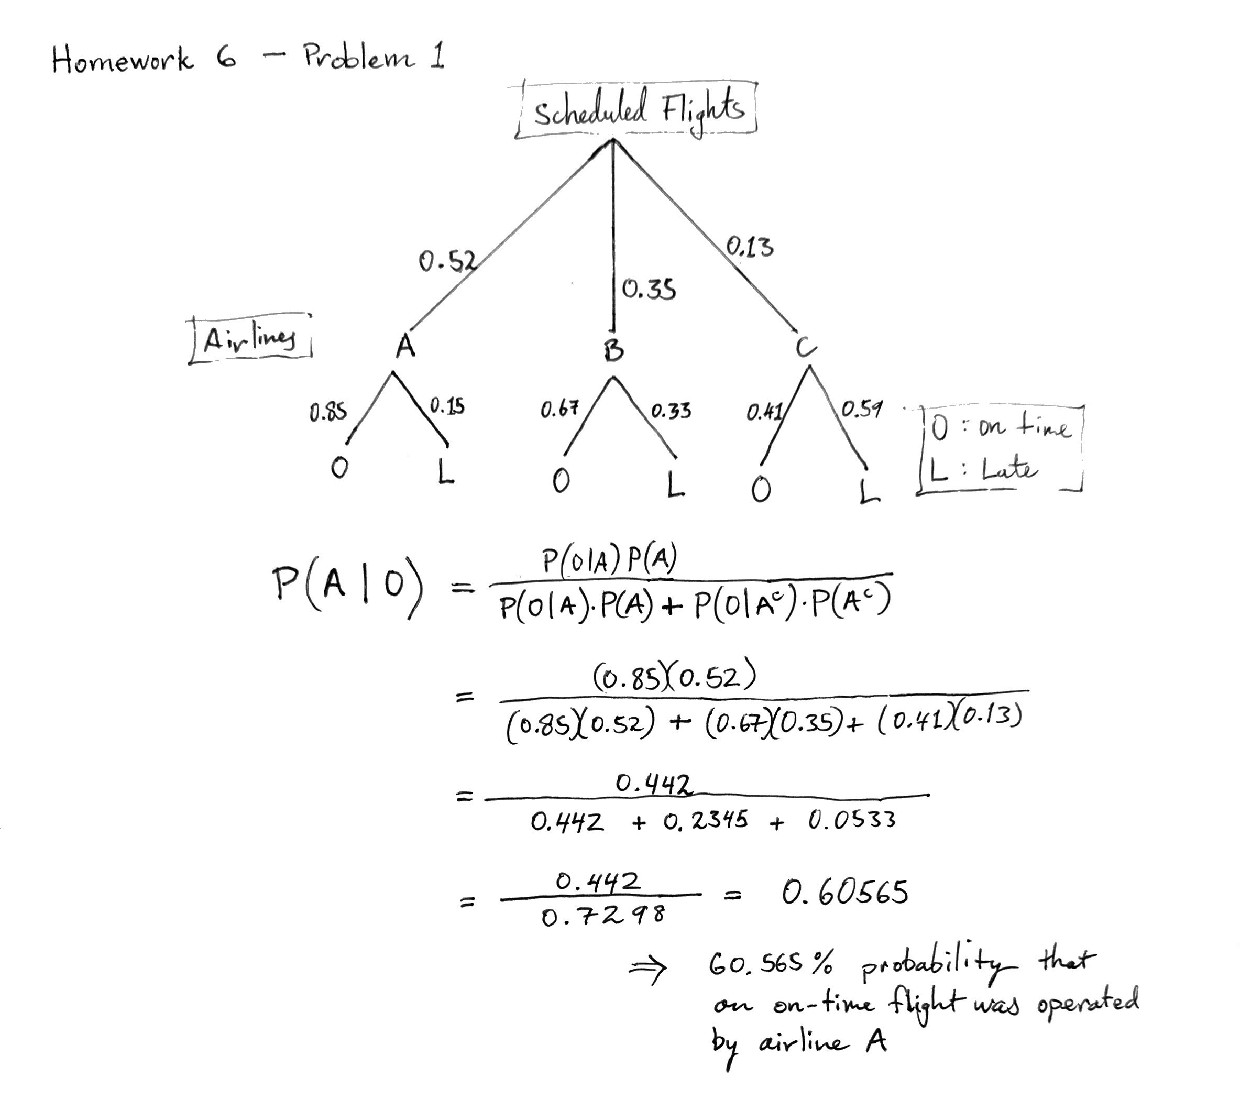
\includegraphics[width=0.75\textwidth,height=\textheight]{/Users/bram/Documents/Math_3190/Homework_6_Data/3190_HW6_Prob1.pdf}
\caption{Problem 1 response}\label{id}
}
\end{figure}

\hypertarget{problem-2-13-points}{%
\section{Problem 2 (13 points)}\label{problem-2-13-points}}

Suppose we have a data set with each observation \(x_i\) independent and
identically exponentially distributed for \(i=1,2,\dots,n\). That is,
\(x_i\sim \text{Exp}(\lambda)\) where \(\lambda\) is the rate parameter.
We would like to find a posterior (or at least a function proportional
to it) for \(\lambda\).

\hypertarget{part-a-5-points}{%
\subsubsection{Part a (5 points)}\label{part-a-5-points}}

Write down the likelihood function (or a function proportional to it) in
this situation. We would call this \(p(x|\lambda)\).

\hypertarget{part-b-5-points}{%
\subsubsection{Part b (5 points)}\label{part-b-5-points}}

Now let \(\lambda\) have a normal prior with mean 0.1 and variance 1:
\(\lambda\sim N(1/10, 1)\). Use this and the likelihood from part a to
write down a function that is proportional to the posterior of
\(\lambda\) given \(\boldsymbol{x}\). We call this
\(p(\lambda|\boldsymbol{x})\).

\begin{figure}
\centering
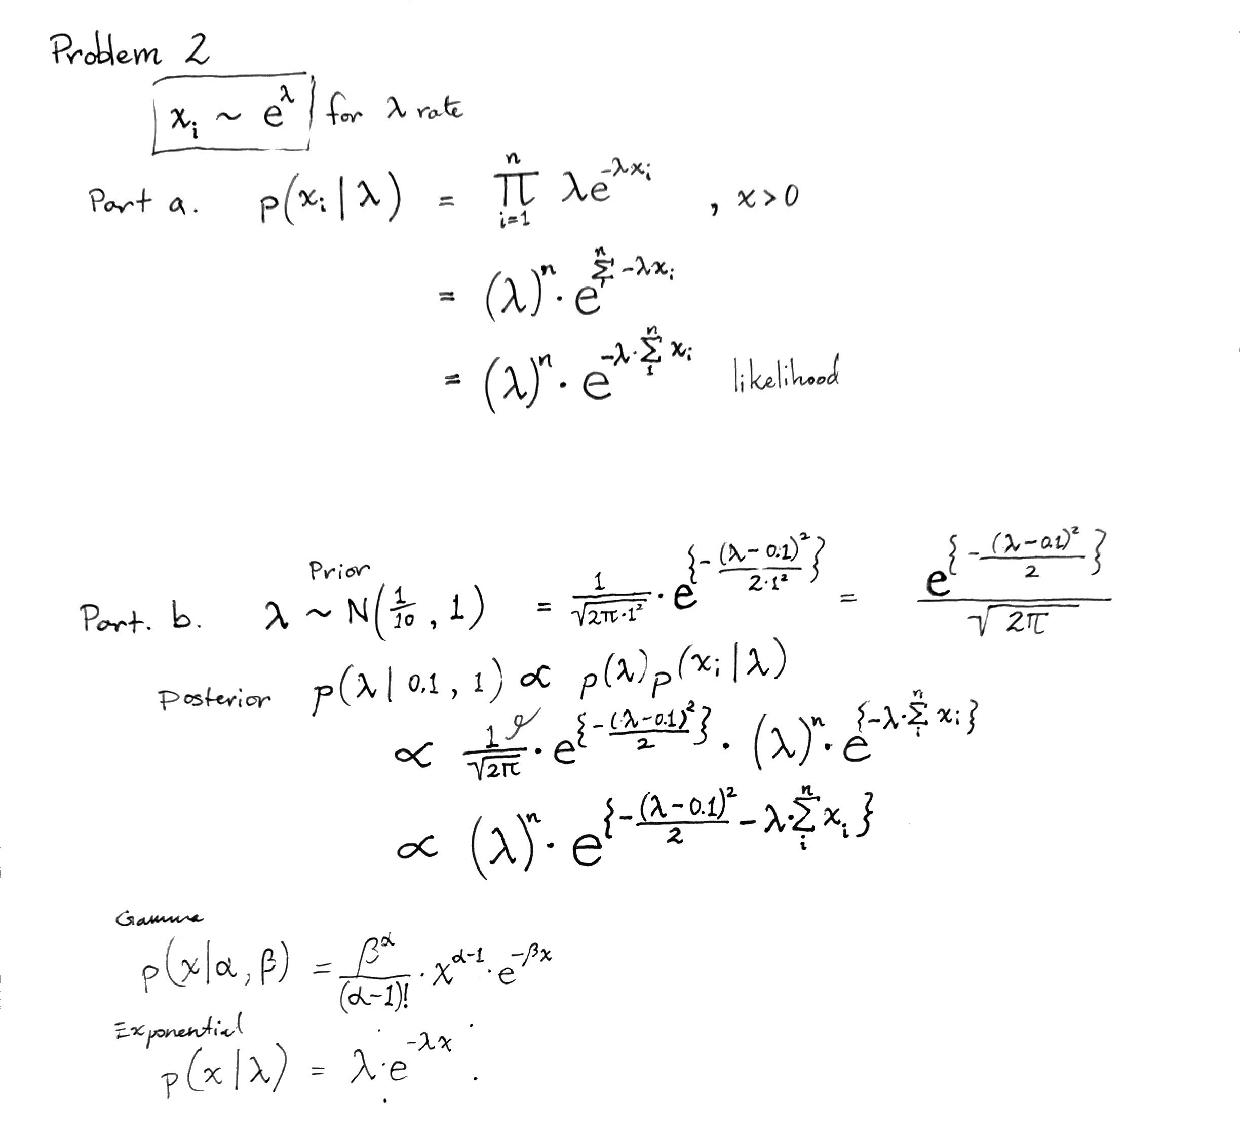
\includegraphics[width=0.75\textwidth,height=\textheight]{/Users/bram/Documents/Math_3190/Homework_6_Data/3190_HW6_Prob2.pdf}
\caption{Problem 2 response}
\end{figure}

\hypertarget{part-c-3-points}{%
\subsubsection{Part c (3 points)}\label{part-c-3-points}}

Which would be more appropriate here to obtain samples of \(\lambda\),
the Gibbs or Metropolis algorithm? Explain why. You may want to look on
page 8 of Notes 8 in the conjugate prior table.

\textbf{Response}: The posterior and its kernel, in this case the entire
expression, does not take the form of any properly defined conjugate. In
this particular case, the Metropolis algorithm will be more appropriate,
setting a symmetric distribution to sample from and using a random
tolerance.

\hypertarget{problem-3-26-points}{%
\section{Problem 3 (26 points)}\label{problem-3-26-points}}

Suppose we have the vector
\texttt{x\ =\ c(1.83,\ 1.72,\ 2.13,\ 2.49,\ 0.90,\ 2.01,\ 1.51,\ 3.12,\ 1.29,\ 1.54,\ 2.94,\ 3.02,\ 0.93,\ 2.78)}
that we believe comes from a gamma distribution with shape of 10 and
some rate \(\beta\): \(x_i\sim\text{Gam}(10,\beta)\). We will use
sampling to obtain some information about \(\beta\). Let's put a gamma
prior on \(\beta\) with a shape of \(\alpha_0\) and a rate of 1:
\(\beta\sim\text{Gam}(\alpha_0,1)\).

\hypertarget{part-a-5-points-1}{%
\subsubsection{Part a (5 points)}\label{part-a-5-points-1}}

Use the fact that this is a conjugate prior to write down what kind of
distribution the posterior of \(\beta\), which is
\(p(\beta|\boldsymbol{x})\), is.

\begin{figure}
\centering
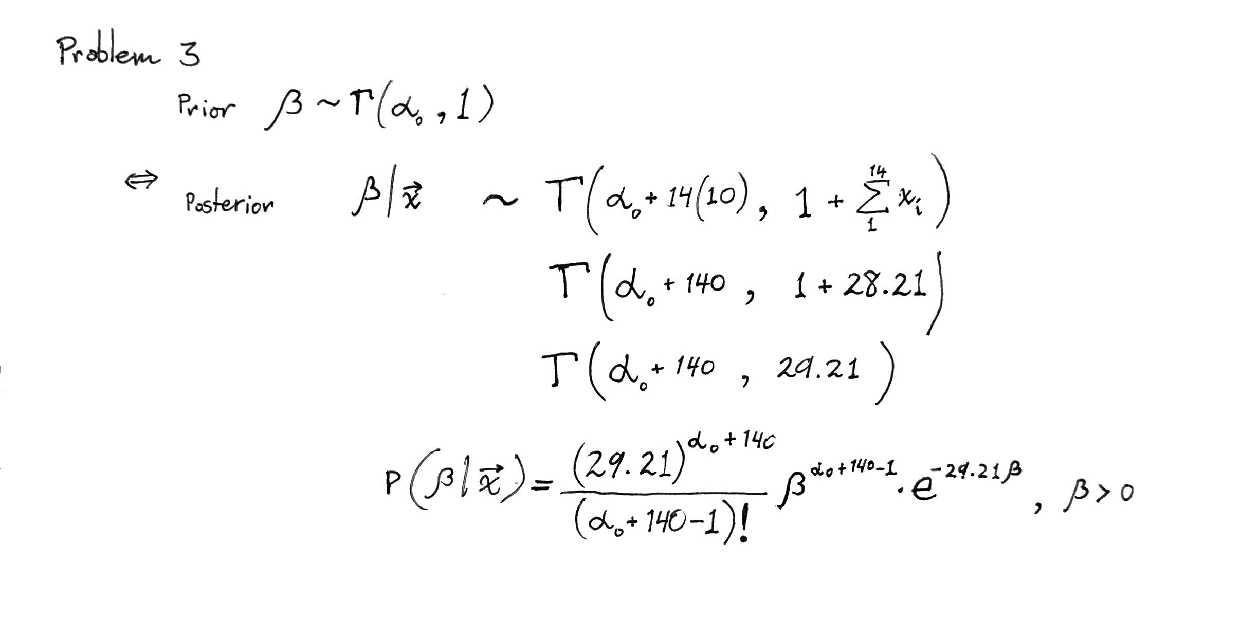
\includegraphics[width=0.75\textwidth,height=\textheight]{/Users/bram/Documents/Math_3190/Homework_6_Data/3190_HW6_Prob3.pdf}
\caption{Problem 3 response}
\end{figure}

\hypertarget{part-b-5-points-1}{%
\subsubsection{Part b (5 points)}\label{part-b-5-points-1}}

Let \(\alpha_0=1\). In an \textbf{R} code chunk, sample 10,000 \(\beta\)
values from the distribution you wrote down in part a using the
\texttt{rgamma()} function and report the 95\% credible interval for
\(\beta\) using the 2.5th and 97.5th percentiles.

\begin{Shaded}
\begin{Highlighting}[]
\FunctionTok{set.seed}\NormalTok{(}\DecValTok{2024}\NormalTok{)}
\NormalTok{x }\OtherTok{\textless{}{-}} \FunctionTok{c}\NormalTok{(}\FloatTok{1.83}\NormalTok{, }\FloatTok{1.72}\NormalTok{, }\FloatTok{2.13}\NormalTok{, }\FloatTok{2.49}\NormalTok{, }\FloatTok{0.90}\NormalTok{, }\FloatTok{2.01}\NormalTok{, }\FloatTok{1.51}\NormalTok{, }
       \FloatTok{3.12}\NormalTok{, }\FloatTok{1.29}\NormalTok{, }\FloatTok{1.54}\NormalTok{, }\FloatTok{2.94}\NormalTok{, }\FloatTok{3.02}\NormalTok{, }\FloatTok{0.93}\NormalTok{, }\FloatTok{2.78}\NormalTok{)}

\NormalTok{alpha\_0 }\OtherTok{\textless{}{-}} \DecValTok{1}

\NormalTok{shape }\OtherTok{\textless{}{-}}\NormalTok{ alpha\_0 }\SpecialCharTok{+} \FunctionTok{length}\NormalTok{(x)}\SpecialCharTok{*}\DecValTok{10}
\NormalTok{rate }\OtherTok{\textless{}{-}} \DecValTok{1} \SpecialCharTok{+} \FunctionTok{sum}\NormalTok{(x)}

\NormalTok{beta }\OtherTok{\textless{}{-}} \FunctionTok{rgamma}\NormalTok{(}\DecValTok{10000}\NormalTok{, shape, rate)}

\FunctionTok{quantile}\NormalTok{(beta, }\FunctionTok{c}\NormalTok{(}\FloatTok{0.025}\NormalTok{, }\FloatTok{0.975}\NormalTok{))}
\end{Highlighting}
\end{Shaded}

\begin{verbatim}
##     2.5%    97.5% 
## 4.056263 5.660807
\end{verbatim}

\textbf{Response}: There is a \(95\%\) chance that \(\beta\) lies in the
interval \([4.058, 5.627]\).

\hypertarget{part-c-3-points-1}{%
\subsubsection{Part c (3 points)}\label{part-c-3-points-1}}

Repeat part b with \(\alpha_0 = 10\).

\begin{Shaded}
\begin{Highlighting}[]
\NormalTok{alpha\_0 }\OtherTok{\textless{}{-}} \DecValTok{10}

\NormalTok{shape }\OtherTok{\textless{}{-}}\NormalTok{ alpha\_0 }\SpecialCharTok{+} \FunctionTok{length}\NormalTok{(x)}\SpecialCharTok{*}\DecValTok{10}
\NormalTok{rate }\OtherTok{\textless{}{-}} \DecValTok{1} \SpecialCharTok{+} \FunctionTok{sum}\NormalTok{(x)}

\NormalTok{beta }\OtherTok{\textless{}{-}} \FunctionTok{rgamma}\NormalTok{(}\DecValTok{10000}\NormalTok{, shape, rate)}

\FunctionTok{quantile}\NormalTok{(beta, }\FunctionTok{c}\NormalTok{(}\FloatTok{0.025}\NormalTok{, }\FloatTok{0.975}\NormalTok{))}
\end{Highlighting}
\end{Shaded}

\begin{verbatim}
##     2.5%    97.5% 
## 4.365546 5.985813
\end{verbatim}

\textbf{Response}: There is a \(95\%\) chance that \(\beta\) lies in the
interval \([4.354, 5.992]\).

\hypertarget{part-d-3-points}{%
\subsubsection{Part d (3 points)}\label{part-d-3-points}}

Repeat part b with \(\alpha_0 = 100\).

\begin{Shaded}
\begin{Highlighting}[]
\NormalTok{alpha\_0 }\OtherTok{\textless{}{-}} \DecValTok{100}

\NormalTok{shape }\OtherTok{\textless{}{-}}\NormalTok{ alpha\_0 }\SpecialCharTok{+} \FunctionTok{length}\NormalTok{(x)}\SpecialCharTok{*}\DecValTok{10}
\NormalTok{rate }\OtherTok{\textless{}{-}} \DecValTok{1} \SpecialCharTok{+} \FunctionTok{sum}\NormalTok{(x)}

\NormalTok{beta }\OtherTok{\textless{}{-}} \FunctionTok{rgamma}\NormalTok{(}\DecValTok{10000}\NormalTok{, shape, rate)}

\FunctionTok{quantile}\NormalTok{(beta, }\FunctionTok{c}\NormalTok{(}\FloatTok{0.025}\NormalTok{, }\FloatTok{0.975}\NormalTok{))}
\end{Highlighting}
\end{Shaded}

\begin{verbatim}
##     2.5%    97.5% 
## 7.220025 9.300305
\end{verbatim}

\textbf{Response}: There is a \(95\%\) chance that \(\beta\) lies in the
interval \([7.226, 9.300]\).

\hypertarget{part-e-7-points}{%
\subsubsection{Part e (7 points)}\label{part-e-7-points}}

Now suppose we have twice as much data (given in the \textbf{R} code
chunk below). Repeat parts b, c, and d using this \texttt{x} vector
instead and report the three 95\% credible intervals. Note, this new
vector x will change the shape and rate parameters used in the
\texttt{rgamma()} functions.

\begin{Shaded}
\begin{Highlighting}[]
\NormalTok{x }\OtherTok{\textless{}{-}} \FunctionTok{c}\NormalTok{(}\FloatTok{1.83}\NormalTok{, }\FloatTok{1.72}\NormalTok{, }\FloatTok{2.13}\NormalTok{, }\FloatTok{2.49}\NormalTok{, }\FloatTok{0.90}\NormalTok{, }\FloatTok{2.01}\NormalTok{, }\FloatTok{1.51}\NormalTok{, }\FloatTok{3.12}\NormalTok{, }\FloatTok{1.29}\NormalTok{, }\FloatTok{1.54}\NormalTok{,}
       \FloatTok{2.94}\NormalTok{, }\FloatTok{3.02}\NormalTok{, }\FloatTok{0.93}\NormalTok{, }\FloatTok{2.78}\NormalTok{, }\FloatTok{2.76}\NormalTok{, }\FloatTok{1.70}\NormalTok{, }\FloatTok{1.42}\NormalTok{, }\FloatTok{2.16}\NormalTok{, }\FloatTok{1.07}\NormalTok{, }\FloatTok{2.21}\NormalTok{,}
       \FloatTok{2.38}\NormalTok{, }\FloatTok{2.27}\NormalTok{, }\FloatTok{1.72}\NormalTok{, }\FloatTok{1.44}\NormalTok{, }\FloatTok{1.54}\NormalTok{, }\FloatTok{1.72}\NormalTok{, }\FloatTok{1.87}\NormalTok{, }\FloatTok{1.39}\NormalTok{)}

\NormalTok{alpha\_values }\OtherTok{\textless{}{-}} \FunctionTok{c}\NormalTok{(}\DecValTok{1}\NormalTok{, }\DecValTok{10}\NormalTok{, }\DecValTok{100}\NormalTok{)}

\CommentTok{\#credible intervals}
\NormalTok{credible\_interval }\OtherTok{\textless{}{-}} \ControlFlowTok{function}\NormalTok{(alpha\_0, x) \{}
\NormalTok{  shape }\OtherTok{\textless{}{-}}\NormalTok{ alpha\_0 }\SpecialCharTok{+} \FunctionTok{length}\NormalTok{(x) }\SpecialCharTok{*} \DecValTok{10}
\NormalTok{  rate }\OtherTok{\textless{}{-}} \DecValTok{1} \SpecialCharTok{+} \FunctionTok{sum}\NormalTok{(x)}
\NormalTok{  beta }\OtherTok{\textless{}{-}} \FunctionTok{rgamma}\NormalTok{(}\DecValTok{10000}\NormalTok{, shape, rate)}
\NormalTok{  interval }\OtherTok{\textless{}{-}} \FunctionTok{quantile}\NormalTok{(beta, }\FunctionTok{c}\NormalTok{(}\FloatTok{0.025}\NormalTok{, }\FloatTok{0.975}\NormalTok{))}
  \FunctionTok{return}\NormalTok{(interval)}
\NormalTok{\}}

\CommentTok{\#intervals for each alpha\_0}
\NormalTok{results }\OtherTok{\textless{}{-}} \FunctionTok{map\_df}\NormalTok{(alpha\_values, }\SpecialCharTok{\textasciitilde{}}\NormalTok{\{}
\NormalTok{  alpha\_0 }\OtherTok{\textless{}{-}}\NormalTok{ .x}
\NormalTok{  interval }\OtherTok{\textless{}{-}} \FunctionTok{credible\_interval}\NormalTok{(alpha\_0, x)}
  \FunctionTok{data.frame}\NormalTok{(}\AttributeTok{alpha\_0 =}\NormalTok{ alpha\_0, }
             \AttributeTok{interval\_lower =}\NormalTok{ interval[}\DecValTok{1}\NormalTok{],  }\CommentTok{\# Extract lower bound}
             \AttributeTok{interval\_upper =}\NormalTok{ interval[}\DecValTok{2}\NormalTok{])  }\CommentTok{\# Extract upper bound}
\NormalTok{\})}

\CommentTok{\#intervals as strings}
\NormalTok{results}\SpecialCharTok{$}\NormalTok{interval\_str }\OtherTok{\textless{}{-}} \FunctionTok{sprintf}\NormalTok{(}\StringTok{"[\%.3f, \%.3f]"}\NormalTok{, results}\SpecialCharTok{$}\NormalTok{interval\_lower, results}\SpecialCharTok{$}\NormalTok{interval\_upper)}


\NormalTok{results }\SpecialCharTok{|\textgreater{}} 
  \FunctionTok{rownames\_to\_column}\NormalTok{(}\AttributeTok{var =} \StringTok{"row\_id"}\NormalTok{) }\SpecialCharTok{|\textgreater{}} 
  \FunctionTok{select}\NormalTok{(}\SpecialCharTok{{-}}\FunctionTok{c}\NormalTok{(interval\_lower, interval\_upper, row\_id)) }\SpecialCharTok{|\textgreater{}} \CommentTok{\#retirer la merde}
  \FunctionTok{kable}\NormalTok{(}\AttributeTok{col.names =} \FunctionTok{c}\NormalTok{(}\StringTok{"⍺\_0"}\NormalTok{, }\StringTok{"Credible Interval"}\NormalTok{)) }\SpecialCharTok{|\textgreater{}} 
  \FunctionTok{kable\_styling}\NormalTok{(}\AttributeTok{full\_width =} \ConstantTok{FALSE}\NormalTok{) }\SpecialCharTok{|\textgreater{}} 
  \FunctionTok{column\_spec}\NormalTok{(}\DecValTok{2}\NormalTok{, }\AttributeTok{bold =} \ConstantTok{TRUE}\NormalTok{)}
\end{Highlighting}
\end{Shaded}

\begin{longtable}[t]{r>{}l}
\toprule
⍺\_0 & Credible Interval\\
\midrule
1 & \textbf{{}[4.535, 5.740]}\\
10 & \textbf{{}[4.690, 5.928]}\\
100 & \textbf{{}[6.234, 7.650]}\\
\bottomrule
\end{longtable}

\hypertarget{part-f-3-points}{%
\subsubsection{Part f (3 points)}\label{part-f-3-points}}

In this problem, the true \(\beta\) value is 5. Write a sentence or two
about the effect adding more data has to these credible intervals by
comparing the intervals from parts b-d to the intervals from part e.

\textbf{Response}: The increased sample data reduced the range of each
credible interval, and in the case of the \(\alpha_0 = 1\) and \(10\)
the interval was closer to and more centered over the true \(\beta=5\).
Where \(\alpha_0 = 100\) the interval \([7.226, 9.300]\) was not
re-centered over \(5\), but reduced and drawn more closely to the true
\(\beta\) by the interval \([6.240,7.634]\).

\hypertarget{problem-4-51-points}{%
\section{Problem 4 (51 points)}\label{problem-4-51-points}}

Let's apply the Bayesian framework to a regression problem. In the
GitHub data folder, there is a file called \texttt{treeseeds.txt} that
contains information about species of tree, the count of seeds it
produces, and the average weight of those seeds in \(mg\).

\hypertarget{part-a-3-points}{%
\subsubsection{Part a (3 points)}\label{part-a-3-points}}

Read in the \texttt{treeseeds.txt} file and take the log of the counts
and weights. Fit an OLS regression model using log(weight) to predict
log(count).

\begin{Shaded}
\begin{Highlighting}[]
\NormalTok{treeseeds }\OtherTok{\textless{}{-}} \FunctionTok{read\_csv}\NormalTok{(}
  \FunctionTok{paste0}\NormalTok{(}\StringTok{"/Users/bram/Documents/Math\_3190/Homework\_6\_Data/treeseeds.txt"}\NormalTok{))}
\end{Highlighting}
\end{Shaded}

\begin{verbatim}
## Rows: 19 Columns: 3
## -- Column specification -------------------------------
## Delimiter: ","
## chr (1): species
## dbl (2): count, weight
## 
## i Use `spec()` to retrieve the full column specification for this data.
## i Specify the column types or set `show_col_types = FALSE` to quiet this message.
\end{verbatim}

\begin{Shaded}
\begin{Highlighting}[]
\NormalTok{treeseeds\_log }\OtherTok{\textless{}{-}}\NormalTok{ treeseeds }\SpecialCharTok{|\textgreater{}} 
  \FunctionTok{mutate}\NormalTok{(}\AttributeTok{ln\_count =} \FunctionTok{log}\NormalTok{(count), }\AttributeTok{ln\_weight =} \FunctionTok{log}\NormalTok{(weight)) }\SpecialCharTok{|\textgreater{}} 
  \FunctionTok{select}\NormalTok{(}\SpecialCharTok{{-}}\NormalTok{count, }\SpecialCharTok{{-}}\NormalTok{weight)}

\NormalTok{treeseeds\_mod }\OtherTok{\textless{}{-}} \FunctionTok{glm}\NormalTok{(ln\_count}\SpecialCharTok{\textasciitilde{}}\NormalTok{ln\_weight, }\AttributeTok{data =}\NormalTok{ treeseeds\_log, }\AttributeTok{family =} \StringTok{"gaussian"}\NormalTok{)}

\FunctionTok{summary}\NormalTok{(treeseeds\_mod)}
\end{Highlighting}
\end{Shaded}

\begin{verbatim}
## 
## Call:
## glm(formula = ln_count ~ ln_weight, family = "gaussian", data = treeseeds_log)
## 
## Coefficients:
##             Estimate Std. Error t value Pr(>|t|)    
## (Intercept)  9.37903    0.39720  23.613 1.95e-14 ***
## ln_weight   -0.51491    0.07185  -7.166 1.58e-06 ***
## ---
## Signif. codes:  
## 0 '***' 0.001 '**' 0.01 '*' 0.05 '.' 0.1 ' ' 1
## 
## (Dispersion parameter for gaussian family taken to be 0.8766687)
## 
##     Null deviance: 59.921  on 18  degrees of freedom
## Residual deviance: 14.903  on 17  degrees of freedom
## AIC: 55.305
## 
## Number of Fisher Scoring iterations: 2
\end{verbatim}

\hypertarget{part-b-15-points}{%
\subsubsection{Part b (15 points)}\label{part-b-15-points}}

We will walk through the mathematics of obtaining the posterior together
here since this problem will focus on coding the Metropolis algorithm.
Assuming the true errors are normal with mean 0 and variance
\(\sigma^2\), \(\epsilon_i\sim N(0,\sigma^2)\), it can be shown that
each \(y_i\) has the distribution \[
p(y_i|x_i,\beta_0,\beta_1,\sigma^2) = \frac{1}{\sqrt{2\pi\sigma^2}}\exp\left(
-\frac{1}{2\sigma^2}(y_i-\beta_0-\beta_1x_i)^2\right)
\]

So, we can write the likelihood is \[
p(y_i|x_i,\beta_0,\beta_1,\sigma^2) \propto\exp\left(
-\frac{1}{2\sigma^2}(y_i-\beta_0-\beta_1x_i)^2\right)
\] where \(y_i\) is the log(count) for observation \(i\) and \(x_i\) is
the log(weight) for observation \(i\). Note that here we think of
\(\boldsymbol{y}\) as being random and \(\boldsymbol{x}\) as being
fixed. We could, in theory, think of the vector \(\boldsymbol{x}\) as
also being random and put a prior on it. But we won't do that here.

Now, let's just put uniform priors on \(\beta_0\) and \(\beta_1\) so the
priors are proportional to 1. Also, let's assume \(\sigma^2=1\). This
seems reasonable since \(s_e^2\), the MSE, is 0.877. Of course, we could
put a prior on \(\sigma^2\) as well and sample it too, but we will focus
on only sampling \(\beta_0\) and \(\beta_1\).

Now, with those uniform priors, and plugging in 1 for \(\sigma^2\), we
have that the joint posterior of \(\beta_0\) and \(\beta_1\) is: \[
p(\beta_0,\beta_1|\boldsymbol{x},\boldsymbol{y}) \propto\exp\left(
-\frac{1}{2}\sum_{i=1}^n(y_i-\beta_0-\beta_1x_i)^2\right)=f(\beta_0,\beta_1|\boldsymbol{x},\boldsymbol{y}).
\]

Then, we can take the log to get \[
\ln(f(\beta_0,\beta_1|\boldsymbol{x},\boldsymbol{y}))=-\frac{1}{2}\sum_{i=1}^n(y_i-\beta_0-\beta_1x_i)^2.
\]

Our goal now is to obtain samples of \(\beta_0\) and \(\beta_1\). Let's
use the Metropolis algorithm to do this. Using the log of the function
proportional to the joint posterior of \(\beta_0\) and \(\beta_1\),
\(\ln(f(\beta_0,\beta_1|\boldsymbol{x},\boldsymbol{y})))\), write a
Metropolis algorithm in \textbf{R}. For \(\beta_0\), you can use a
normal proposal distribution centered at the previous value,
\(\beta_0^{(i)}\), with a standard deviation of 0.8 and for \(\beta_1\),
you can use a normal proposal distribution centered at the previous
value, \(\beta_1^{(i)}\), with a standard deviation of 0.1. The starting
values don't matter too much, but we can use \(\beta_0^{(0)}=10\) and
\(\beta_1^{(0)}=-0.5\). It may be useful to look at the
\texttt{Notes\ 8\ Script.R} file that is on GitHub in the Notes 8 folder
and is on Canvas.

Obtain at least 10,000 samples (set a seed, please) and plot the chains
for \(\beta_0\) and \(\beta_1\). For this problem, include:

\begin{enumerate}
\def\labelenumi{\arabic{enumi}.}
\tightlist
\item
  The plot for the \(\beta_0\) chain.
\item
  The plot for the \(\beta_1\) chain.
\item
  The 95\% credible interval for \(\beta_0\) based on the 2.5th and
  97.5th percentiles.
\item
  The 95\% credible interval for \(\beta_1\) based on the 2.5th and
  97.5th percentiles.
\end{enumerate}

\begin{Shaded}
\begin{Highlighting}[]
\NormalTok{joint\_function }\OtherTok{\textless{}{-}} \ControlFlowTok{function}\NormalTok{(y, x, b\_0, b\_1) \{}
\NormalTok{  arg }\OtherTok{\textless{}{-}}\NormalTok{ y }\SpecialCharTok{{-}}\NormalTok{ b\_0 }\SpecialCharTok{{-}}\NormalTok{ b\_1 }\SpecialCharTok{*}\NormalTok{ x}
\NormalTok{  arg2 }\OtherTok{\textless{}{-}}\NormalTok{ arg}\SpecialCharTok{\^{}}\DecValTok{2}
\NormalTok{  result }\OtherTok{\textless{}{-}}\NormalTok{ (}\SpecialCharTok{{-}}\DecValTok{1}\SpecialCharTok{/}\DecValTok{2}\NormalTok{) }\SpecialCharTok{*} \FunctionTok{sum}\NormalTok{(arg2)}
  \FunctionTok{return}\NormalTok{(result)}
\NormalTok{\}}

\FunctionTok{set.seed}\NormalTok{(}\DecValTok{2024}\NormalTok{)}

\NormalTok{n\_samps }\OtherTok{\textless{}{-}} \DecValTok{10000}
\NormalTok{beta\_0 }\OtherTok{\textless{}{-}} \FunctionTok{rep}\NormalTok{(}\DecValTok{0}\NormalTok{, n\_samps)}
\NormalTok{beta\_1 }\OtherTok{\textless{}{-}} \FunctionTok{rep}\NormalTok{(}\DecValTok{0}\NormalTok{,n\_samps)}

\NormalTok{beta\_0[}\DecValTok{1}\NormalTok{] }\OtherTok{\textless{}{-}} \DecValTok{10}
\NormalTok{beta\_1[}\DecValTok{1}\NormalTok{] }\OtherTok{\textless{}{-}} \SpecialCharTok{{-}}\FloatTok{0.5}

\NormalTok{n }\OtherTok{\textless{}{-}} \FunctionTok{length}\NormalTok{(treeseeds) }

\ControlFlowTok{for}\NormalTok{ (i }\ControlFlowTok{in} \DecValTok{1}\SpecialCharTok{:}\NormalTok{(n\_samps }\SpecialCharTok{{-}} \DecValTok{1}\NormalTok{)) \{}
\NormalTok{  beta\_0\_star }\OtherTok{\textless{}{-}} \FunctionTok{rnorm}\NormalTok{(}\DecValTok{1}\NormalTok{, beta\_0[i], }\FloatTok{0.8}\NormalTok{)}
\NormalTok{  beta\_1\_star }\OtherTok{\textless{}{-}} \FunctionTok{rnorm}\NormalTok{(}\DecValTok{1}\NormalTok{, beta\_1[i], }\FloatTok{0.1}\NormalTok{)}
  
\CommentTok{\# using the natural log of the proportional joint posterior distribution of ß\_0, ß\_1 as function:}
  
  \DocumentationTok{\#\#for the ratio R numerator f(Ø*|x) (is logged for difference)}
\NormalTok{  ln\_f1 }\OtherTok{\textless{}{-}} \FunctionTok{joint\_function}\NormalTok{(treeseeds\_log}\SpecialCharTok{$}\NormalTok{ln\_count, treeseeds\_log}\SpecialCharTok{$}\NormalTok{ln\_weight, beta\_0\_star, beta\_1\_star)}
  
  \DocumentationTok{\#\# for the ratio R denominator f(Ø\^{}i|x) (is logged for difference)}
\NormalTok{  ln\_f2 }\OtherTok{\textless{}{-}} \FunctionTok{joint\_function}\NormalTok{(treeseeds\_log}\SpecialCharTok{$}\NormalTok{ln\_count, treeseeds\_log}\SpecialCharTok{$}\NormalTok{ln\_weight, beta\_0[i], beta\_1[i])}
  
  \ControlFlowTok{if}\NormalTok{ (}\FunctionTok{log}\NormalTok{(}\FunctionTok{runif}\NormalTok{(}\DecValTok{1}\NormalTok{)) }\SpecialCharTok{\textless{}}\NormalTok{ (ln\_f1 }\SpecialCharTok{{-}}\NormalTok{ ln\_f2)) \{}
\NormalTok{    beta\_0[i}\SpecialCharTok{+}\DecValTok{1}\NormalTok{] }\OtherTok{\textless{}{-}}\NormalTok{ beta\_0\_star}
\NormalTok{    beta\_1[i}\SpecialCharTok{+}\DecValTok{1}\NormalTok{] }\OtherTok{\textless{}{-}}\NormalTok{ beta\_1\_star}
\NormalTok{  \} }\ControlFlowTok{else}\NormalTok{ \{}
\NormalTok{    beta\_0[i}\SpecialCharTok{+}\DecValTok{1}\NormalTok{] }\OtherTok{\textless{}{-}}\NormalTok{ beta\_0[i]}
\NormalTok{    beta\_1[i}\SpecialCharTok{+}\DecValTok{1}\NormalTok{] }\OtherTok{\textless{}{-}}\NormalTok{ beta\_1[i]}
\NormalTok{  \}}
  
\NormalTok{\}}



\CommentTok{\# Sample path plots}
\FunctionTok{ggplot}\NormalTok{(}\FunctionTok{data.frame}\NormalTok{(}\AttributeTok{x =} \DecValTok{1}\SpecialCharTok{:}\NormalTok{n\_samps, beta\_0)) }\SpecialCharTok{+}
  \FunctionTok{geom\_line}\NormalTok{(}\FunctionTok{aes}\NormalTok{(}\AttributeTok{x =}\NormalTok{ x, }\AttributeTok{y =}\NormalTok{ beta\_0), }\AttributeTok{color =} \StringTok{"slategray4"}\NormalTok{, }\AttributeTok{linetype =} \StringTok{"solid"}\NormalTok{) }\SpecialCharTok{+}
  \FunctionTok{labs}\NormalTok{(}\AttributeTok{title =} \FunctionTok{expression}\NormalTok{(}\FunctionTok{paste}\NormalTok{(}\StringTok{"Sample Path of "}\NormalTok{, beta[}\DecValTok{0}\NormalTok{])),}
       \AttributeTok{x =} \StringTok{"Index (Sample Number)"}\NormalTok{, }\AttributeTok{y =} \FunctionTok{expression}\NormalTok{(beta[}\DecValTok{0}\NormalTok{]), }
       \AttributeTok{caption =} \StringTok{""}\NormalTok{, }\AttributeTok{nudge\_y =} \FloatTok{0.1}\NormalTok{) }\SpecialCharTok{+}
  \FunctionTok{theme\_bw}\NormalTok{() }\SpecialCharTok{+}
  \FunctionTok{theme}\NormalTok{(}\AttributeTok{plot.title =} \FunctionTok{element\_text}\NormalTok{(}\AttributeTok{hjust =} \FloatTok{0.5}\NormalTok{))}
\end{Highlighting}
\end{Shaded}

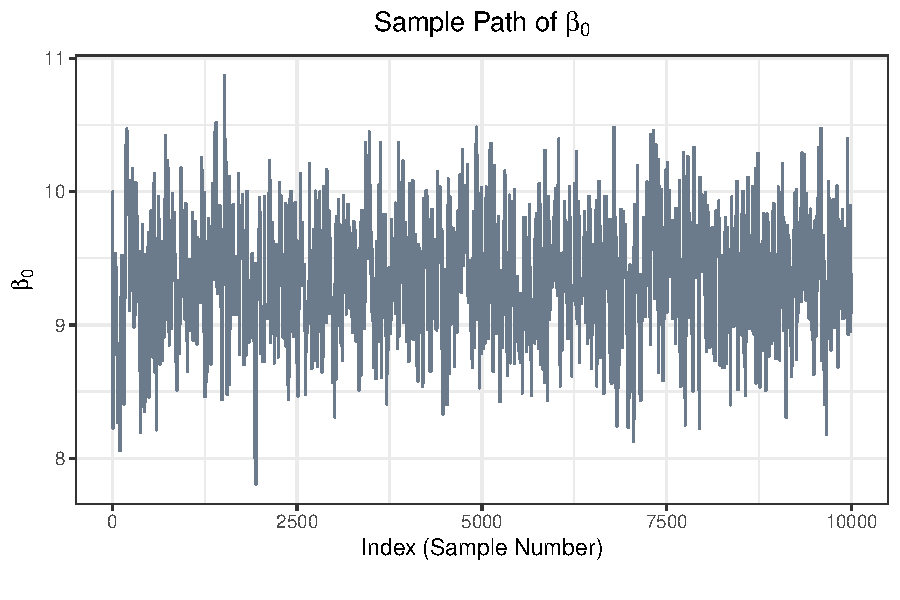
\includegraphics{Homework_6_files/figure-latex/prob4b-1.pdf}

\begin{Shaded}
\begin{Highlighting}[]
\FunctionTok{ggplot}\NormalTok{(}\FunctionTok{data.frame}\NormalTok{(}\AttributeTok{x =} \DecValTok{1}\SpecialCharTok{:}\NormalTok{n\_samps, beta\_1)) }\SpecialCharTok{+}
  \FunctionTok{geom\_line}\NormalTok{(}\FunctionTok{aes}\NormalTok{(}\AttributeTok{x =}\NormalTok{ x, }\AttributeTok{y =}\NormalTok{ beta\_1), }\AttributeTok{color =} \StringTok{"darkorange4"}\NormalTok{, }\AttributeTok{linetype =} \StringTok{"solid"}\NormalTok{) }\SpecialCharTok{+}
  \FunctionTok{labs}\NormalTok{(}\AttributeTok{title =} \FunctionTok{expression}\NormalTok{(}\FunctionTok{paste}\NormalTok{(}\StringTok{"Sample Path of "}\NormalTok{, beta[}\DecValTok{1}\NormalTok{])),}
       \AttributeTok{x =} \StringTok{"Index (Sample Number)"}\NormalTok{, }\AttributeTok{y =} \FunctionTok{expression}\NormalTok{(beta[}\DecValTok{1}\NormalTok{]), }
       \AttributeTok{caption =} \StringTok{""}\NormalTok{, }\AttributeTok{nudge\_y =} \FloatTok{0.1}\NormalTok{) }\SpecialCharTok{+}
  \FunctionTok{theme\_bw}\NormalTok{() }\SpecialCharTok{+}
  \FunctionTok{theme}\NormalTok{(}\AttributeTok{plot.title =} \FunctionTok{element\_text}\NormalTok{(}\AttributeTok{hjust =} \FloatTok{0.5}\NormalTok{))}
\end{Highlighting}
\end{Shaded}

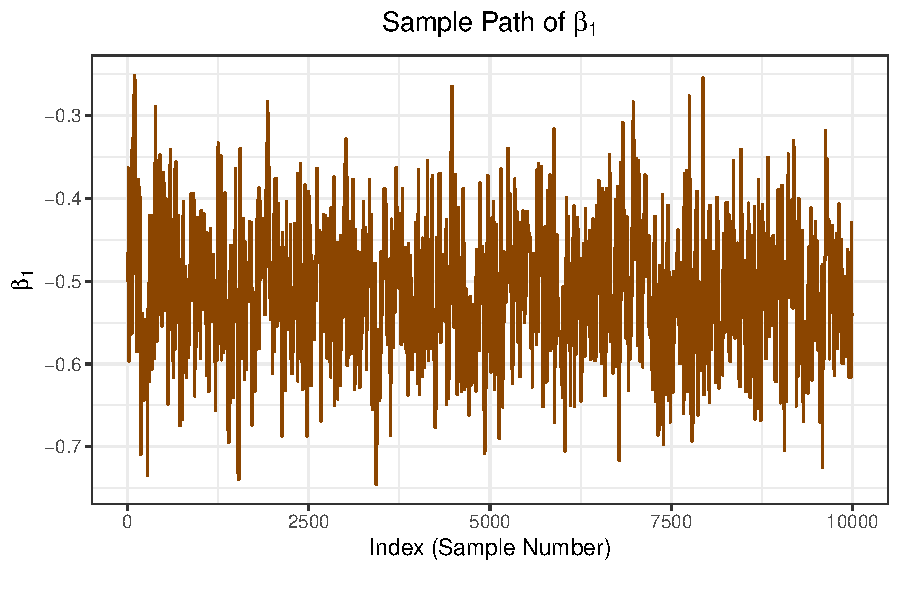
\includegraphics{Homework_6_files/figure-latex/prob4b-2.pdf}

\begin{Shaded}
\begin{Highlighting}[]
\CommentTok{\# Histogram plots}
\FunctionTok{ggplot}\NormalTok{(}\FunctionTok{data.frame}\NormalTok{(beta\_0)) }\SpecialCharTok{+}
  \FunctionTok{geom\_histogram}\NormalTok{(}\FunctionTok{aes}\NormalTok{(}\AttributeTok{x =}\NormalTok{ beta\_0), }\AttributeTok{bins =} \DecValTok{30}\NormalTok{, }\AttributeTok{color =} \StringTok{"slategray3"}\NormalTok{, }\AttributeTok{fill =} \StringTok{"slategray4"}\NormalTok{) }\SpecialCharTok{+}
  \FunctionTok{labs}\NormalTok{(}\AttributeTok{title =} \FunctionTok{expression}\NormalTok{(}\FunctionTok{paste}\NormalTok{(}\FunctionTok{bold}\NormalTok{(}\StringTok{"Histogram of "}\NormalTok{), beta[}\DecValTok{0}\NormalTok{])), }\AttributeTok{x =} \FunctionTok{expression}\NormalTok{(beta[}\DecValTok{0}\NormalTok{]), }\AttributeTok{y =} \StringTok{"Frequency"}\NormalTok{, }\AttributeTok{caption =} \StringTok{""}\NormalTok{) }\SpecialCharTok{+}
  \FunctionTok{theme\_bw}\NormalTok{() }\SpecialCharTok{+}
  \FunctionTok{theme}\NormalTok{(}\AttributeTok{plot.title =} \FunctionTok{element\_text}\NormalTok{(}\AttributeTok{hjust =} \FloatTok{0.5}\NormalTok{))}
\end{Highlighting}
\end{Shaded}

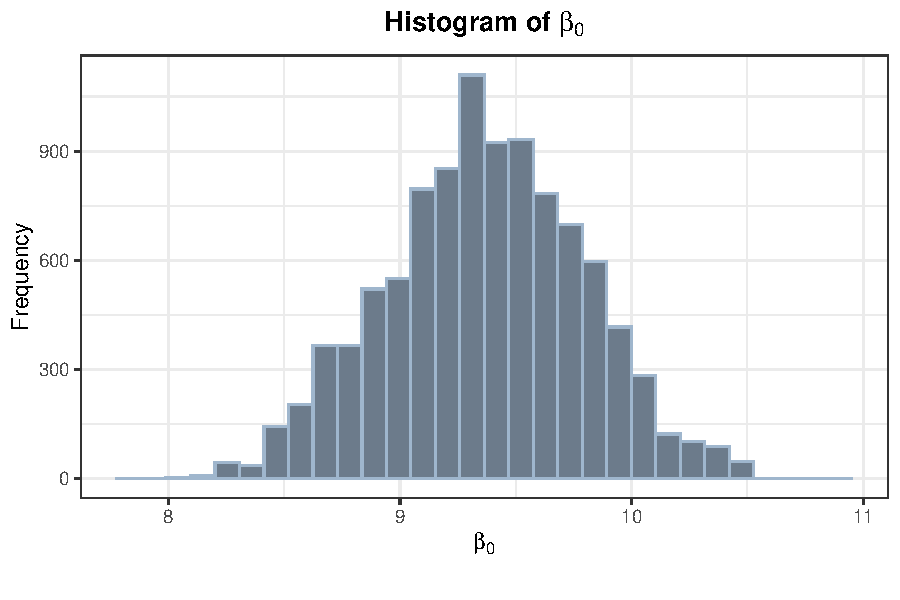
\includegraphics{Homework_6_files/figure-latex/prob4b-3.pdf}

\begin{Shaded}
\begin{Highlighting}[]
\FunctionTok{ggplot}\NormalTok{(}\FunctionTok{data.frame}\NormalTok{(beta\_1)) }\SpecialCharTok{+}
  \FunctionTok{geom\_histogram}\NormalTok{(}\FunctionTok{aes}\NormalTok{(}\AttributeTok{x =}\NormalTok{ beta\_1), }\AttributeTok{bins =} \DecValTok{30}\NormalTok{, }\AttributeTok{color =} \StringTok{"orange1"}\NormalTok{, }\AttributeTok{fill =} \StringTok{"darkorange3"}\NormalTok{) }\SpecialCharTok{+}
  \FunctionTok{labs}\NormalTok{(}\AttributeTok{title =} \FunctionTok{expression}\NormalTok{(}\FunctionTok{paste}\NormalTok{(}\FunctionTok{bold}\NormalTok{(}\StringTok{"Histogram of "}\NormalTok{), beta[}\DecValTok{1}\NormalTok{])), }
       \AttributeTok{x =} \FunctionTok{expression}\NormalTok{(beta[}\DecValTok{1}\NormalTok{]), }\AttributeTok{y =} \StringTok{"Frequency"}\NormalTok{, }
       \AttributeTok{caption =} \StringTok{""}\NormalTok{) }\SpecialCharTok{+}
  \FunctionTok{theme\_bw}\NormalTok{() }\SpecialCharTok{+}
  \FunctionTok{theme}\NormalTok{(}\AttributeTok{plot.title =} \FunctionTok{element\_text}\NormalTok{(}\AttributeTok{hjust =} \FloatTok{0.5}\NormalTok{))}
\end{Highlighting}
\end{Shaded}

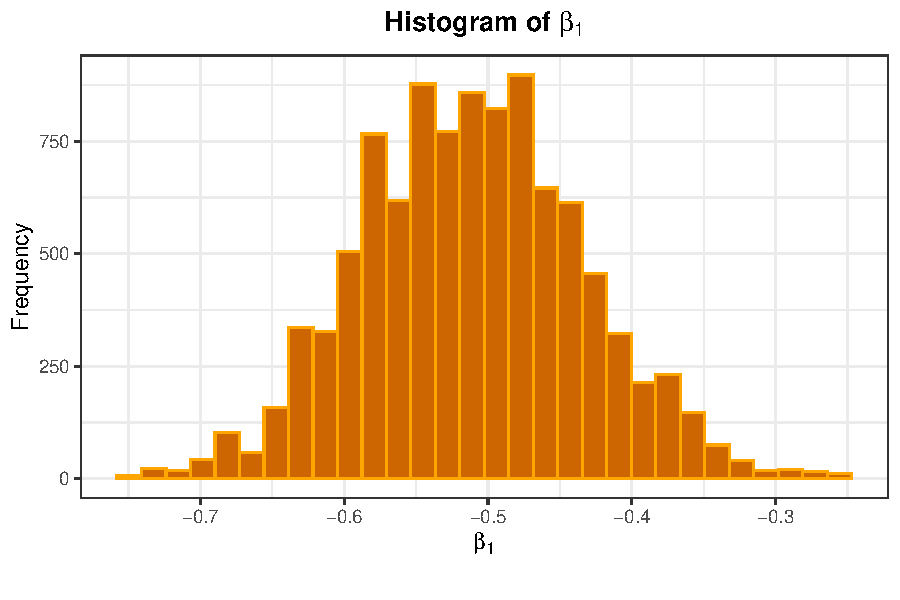
\includegraphics{Homework_6_files/figure-latex/prob4b-4.pdf}

\begin{Shaded}
\begin{Highlighting}[]
\CommentTok{\#quantiles for betas}
\FunctionTok{quantile}\NormalTok{(beta\_0, }\FunctionTok{c}\NormalTok{(}\FloatTok{0.025}\NormalTok{, }\FloatTok{0.975}\NormalTok{))}
\end{Highlighting}
\end{Shaded}

\begin{verbatim}
##      2.5%     97.5% 
##  8.528203 10.199103
\end{verbatim}

\begin{Shaded}
\begin{Highlighting}[]
\FunctionTok{quantile}\NormalTok{(beta\_1, }\FunctionTok{c}\NormalTok{(}\FloatTok{0.025}\NormalTok{, }\FloatTok{0.975}\NormalTok{))}
\end{Highlighting}
\end{Shaded}

\begin{verbatim}
##       2.5%      97.5% 
## -0.6598421 -0.3586130
\end{verbatim}

\begin{Shaded}
\begin{Highlighting}[]
\CommentTok{\#autocorrelation plots for betas}
\FunctionTok{acf}\NormalTok{(beta\_0, }\AttributeTok{main =} \FunctionTok{expression}\NormalTok{(}\FunctionTok{paste}\NormalTok{(}\StringTok{"Autocorrelation of "}\NormalTok{, beta[}\DecValTok{0}\NormalTok{], }\StringTok{" Chain"}\NormalTok{)), }\AttributeTok{mgp =} \FunctionTok{c}\NormalTok{(}\FloatTok{2.7}\NormalTok{, }\DecValTok{1}\NormalTok{, }\DecValTok{0}\NormalTok{), }\AttributeTok{cex.lab =} \FloatTok{1.3}\NormalTok{, }\AttributeTok{lwd =} \DecValTok{3}\NormalTok{)}
\end{Highlighting}
\end{Shaded}

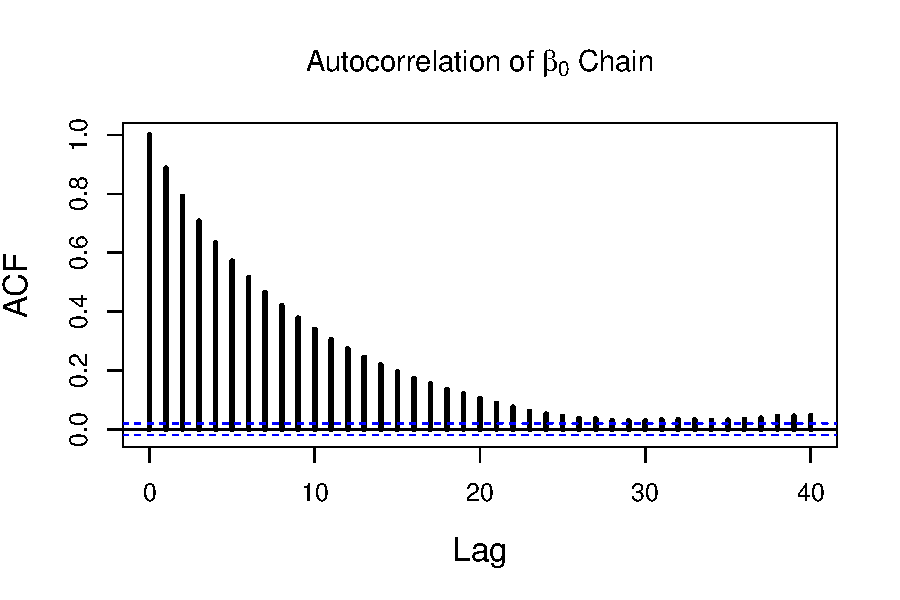
\includegraphics{Homework_6_files/figure-latex/prob4b-5.pdf}

\begin{Shaded}
\begin{Highlighting}[]
\FunctionTok{acf}\NormalTok{(beta\_1, }\AttributeTok{main =} \FunctionTok{expression}\NormalTok{(}\FunctionTok{paste}\NormalTok{(}\StringTok{"Autocorrelation of "}\NormalTok{, beta[}\DecValTok{1}\NormalTok{], }\StringTok{" Chain"}\NormalTok{)), }\AttributeTok{mgp =} \FunctionTok{c}\NormalTok{(}\FloatTok{2.7}\NormalTok{, }\DecValTok{1}\NormalTok{, }\DecValTok{0}\NormalTok{), }\AttributeTok{cex.lab =} \FloatTok{1.3}\NormalTok{, }\AttributeTok{lwd =} \DecValTok{3}\NormalTok{)}
\end{Highlighting}
\end{Shaded}

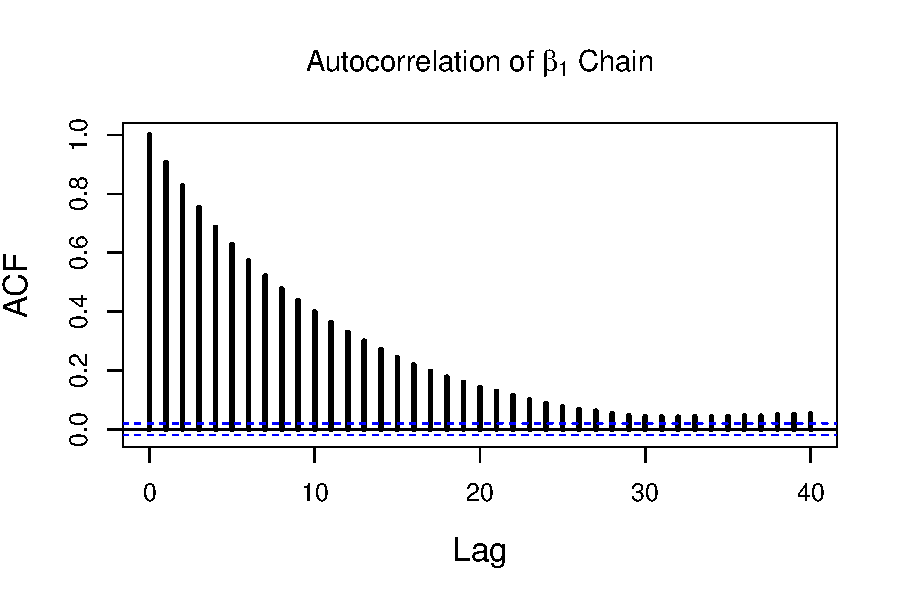
\includegraphics{Homework_6_files/figure-latex/prob4b-6.pdf}

\hypertarget{part-c-3-points-2}{%
\subsubsection{Part c (3 points)}\label{part-c-3-points-2}}

Based on the plots of the chains from part b, does it look like the
Metropolis sampling worked fairly well?

\textbf{Response:} The graph of the sampling chain does not exhibit
strong directional patterns over the 10,000 iterations, suggesting that
there are few iterations which depend on many preceding it. We infer
that the Metropolis sampling worked relatively well.

\hypertarget{part-d-4-points}{%
\subsubsection{Part d (4 points)}\label{part-d-4-points}}

Interpret both of the credible intervals from part b.

\begin{Shaded}
\begin{Highlighting}[]
\NormalTok{cred\_intervals }\OtherTok{\textless{}{-}} \FunctionTok{data.frame}\NormalTok{(}
  \AttributeTok{Parameter\_Variable =} \FunctionTok{c}\NormalTok{(}\StringTok{\textquotesingle{}ß\_0\textquotesingle{}}\NormalTok{, }\StringTok{\textquotesingle{}ß\_1\textquotesingle{}}\NormalTok{),}
  \AttributeTok{Lower\_2.5 =} \FunctionTok{c}\NormalTok{(}\FunctionTok{quantile}\NormalTok{(beta\_0, }\FloatTok{0.025}\NormalTok{), }\FunctionTok{quantile}\NormalTok{(beta\_1, }\FloatTok{0.025}\NormalTok{)),}
  \AttributeTok{Upper\_97.5 =} \FunctionTok{c}\NormalTok{(}\FunctionTok{quantile}\NormalTok{(beta\_0, }\FloatTok{0.975}\NormalTok{), }\FunctionTok{quantile}\NormalTok{(beta\_1, }\FloatTok{0.975}\NormalTok{))}
\NormalTok{)}

\FunctionTok{kable}\NormalTok{(cred\_intervals, }\AttributeTok{format =} \StringTok{"html"}\NormalTok{, }\AttributeTok{align =} \StringTok{"c"}\NormalTok{) }\SpecialCharTok{|\textgreater{}} 
  \FunctionTok{kable\_styling}\NormalTok{(}\AttributeTok{full\_width =} \ConstantTok{FALSE}\NormalTok{)}
\end{Highlighting}
\end{Shaded}

Parameter\_Variable

Lower\_2.5

Upper\_97.5

ß\_0

8.5282034

10.199103

ß\_1

-0.6598421

-0.358613

\textbf{Response:} There is a 95\% chance that the true natural log of
seed counts (intercept \(\beta_0\)) lies in the interval
\([8.528,10.199]\) when the log of seed weights is zero.\\
There is a 95\% chance that the true change in the natural log of seed
counts (slope \(\beta_1\)) lies in the interval \([-0.660, -0.359]\) for
each unit change in the natural log of seed weights.

\hypertarget{part-e-5-points}{%
\subsubsection{Part e (5 points)}\label{part-e-5-points}}

Find and report the integrated autocorrelation time for the \(\beta_0\)
and \(\beta_1\) chains. Each chain will have their own
\(\hat{\tau}_{int}\) value, so you should report two (although they will
be similar).

\begin{Shaded}
\begin{Highlighting}[]
\CommentTok{\#ESS calculations for betas}
\NormalTok{ess\_beta0 }\OtherTok{\textless{}{-}} \DecValTok{1} \SpecialCharTok{+} \DecValTok{2} \SpecialCharTok{*} \FunctionTok{sum}\NormalTok{( }\FunctionTok{abs}\NormalTok{(}\FunctionTok{acf}\NormalTok{(beta\_0, }\AttributeTok{lag.max =} \DecValTok{100}\NormalTok{, }\AttributeTok{plot =}\NormalTok{ F)}\SpecialCharTok{$}\NormalTok{acf) )}
\NormalTok{K\_ESS\_1 }\OtherTok{\textless{}{-}}\NormalTok{ n\_samps}\SpecialCharTok{/}\NormalTok{ess\_beta0}

\NormalTok{ess\_beta1 }\OtherTok{\textless{}{-}} \DecValTok{1} \SpecialCharTok{+} \DecValTok{2} \SpecialCharTok{*} \FunctionTok{sum}\NormalTok{( }\FunctionTok{abs}\NormalTok{(}\FunctionTok{acf}\NormalTok{(beta\_1, }\AttributeTok{lag.max =} \DecValTok{100}\NormalTok{, }\AttributeTok{plot =}\NormalTok{ F)}\SpecialCharTok{$}\NormalTok{acf) ) }
\FunctionTok{print}\NormalTok{(ess\_beta1)}
\end{Highlighting}
\end{Shaded}

\begin{verbatim}
## [1] 25.78817
\end{verbatim}

\begin{Shaded}
\begin{Highlighting}[]
\NormalTok{K\_ESS\_2 }\OtherTok{\textless{}{-}}\NormalTok{ n\_samps}\SpecialCharTok{/}\NormalTok{ess\_beta1}

\FunctionTok{print}\NormalTok{(}\FunctionTok{paste0}\NormalTok{(}\StringTok{\textquotesingle{}Integrated Autocorrelation Time for ß\_0 is \textquotesingle{}}\NormalTok{,}\FunctionTok{round}\NormalTok{(ess\_beta0, }\DecValTok{3}\NormalTok{)))}
\end{Highlighting}
\end{Shaded}

\begin{verbatim}
## [1] "Integrated Autocorrelation Time for ß_0 is 22.709"
\end{verbatim}

\begin{Shaded}
\begin{Highlighting}[]
\FunctionTok{print}\NormalTok{(}\FunctionTok{paste0}\NormalTok{(}\StringTok{\textquotesingle{}Integrated Autocorrelation Time for ß\_1 is \textquotesingle{}}\NormalTok{,}\FunctionTok{round}\NormalTok{(ess\_beta1, }\DecValTok{3}\NormalTok{)))}
\end{Highlighting}
\end{Shaded}

\begin{verbatim}
## [1] "Integrated Autocorrelation Time for ß_1 is 25.788"
\end{verbatim}

\hypertarget{part-f-3-points-1}{%
\subsubsection{Part f (3 points)}\label{part-f-3-points-1}}

Based on the integrated autocorrelation time for the \(\beta_0\) and
\(\beta_1\) chains, how many MCMC samples would you need to generate to
get the equivalent of 10,000 independent samples?

\begin{Shaded}
\begin{Highlighting}[]
\NormalTok{equiv\_ss1 }\OtherTok{\textless{}{-}}\NormalTok{ n\_samps }\SpecialCharTok{*}\NormalTok{ ess\_beta0}
\NormalTok{equiv\_ss2 }\OtherTok{\textless{}{-}}\NormalTok{ n\_samps }\SpecialCharTok{*}\NormalTok{ ess\_beta1}

\FunctionTok{print}\NormalTok{(}\FunctionTok{paste}\NormalTok{(}\StringTok{"ß\_0:"}\NormalTok{, }\FunctionTok{round}\NormalTok{(equiv\_ss1,}\DecValTok{1}\NormalTok{), }\StringTok{"ß\_1:"}\NormalTok{, }\FunctionTok{round}\NormalTok{(equiv\_ss2,}\DecValTok{1}\NormalTok{)))}
\end{Highlighting}
\end{Shaded}

\begin{verbatim}
## [1] "ß_0: 227089.8 ß_1: 257881.7"
\end{verbatim}

Considering the \(\hat\tau_{int}\) for \(\beta_1\), to obtain the
equivalent of 10,000 samples would require the number of MCMC samples to
be at least \(257,882\).

\hypertarget{part-g-3-points}{%
\subsubsection{Part g (3 points)}\label{part-g-3-points}}

Let's compare these credible intervals to some other intervals. First,
obtain the 95\% \(t\) confidence intervals for \(\beta_0\) and
\(\beta_1\) just using the \texttt{confint()} function and report them
here.

\begin{Shaded}
\begin{Highlighting}[]
\NormalTok{ci\_seed\_model }\OtherTok{\textless{}{-}} \FunctionTok{confint}\NormalTok{(treeseeds\_mod)}
\end{Highlighting}
\end{Shaded}

\begin{verbatim}
## Waiting for profiling to be done...
\end{verbatim}

\begin{Shaded}
\begin{Highlighting}[]
\NormalTok{row\_names }\OtherTok{\textless{}{-}} \FunctionTok{c}\NormalTok{(}\StringTok{"ß\_0 (Intercept)"}\NormalTok{, }\StringTok{"ß\_1 (ln\_weight)"}\NormalTok{)}
\FunctionTok{rownames}\NormalTok{(ci\_seed\_model) }\OtherTok{\textless{}{-}}\NormalTok{ row\_names}

\FunctionTok{colnames}\NormalTok{(ci\_seed\_model) }\OtherTok{\textless{}{-}} \FunctionTok{c}\NormalTok{(}\StringTok{"2.5 \%"}\NormalTok{, }\StringTok{"97.5 \%"}\NormalTok{)}

\FunctionTok{kable}\NormalTok{(ci\_seed\_model, }\AttributeTok{format =} \StringTok{"html"}\NormalTok{) }\SpecialCharTok{|\textgreater{}} 
  \FunctionTok{kable\_styling}\NormalTok{(}\AttributeTok{full\_width =} \ConstantTok{FALSE}\NormalTok{) }\SpecialCharTok{|\textgreater{}} 
  \FunctionTok{add\_header\_above}\NormalTok{(}\FunctionTok{c}\NormalTok{(}\StringTok{"Parameter Confidence Intervals"} \OtherTok{=} \DecValTok{3}\NormalTok{))}
\end{Highlighting}
\end{Shaded}

Parameter Confidence Intervals

2.5 \%

97.5 \%

ß\_0 (Intercept)

8.6005353

10.1575170

ß\_1 (ln\_weight)

-0.6557376

-0.3740727

\hypertarget{part-h-10-points}{%
\subsubsection{Part h (10 points)}\label{part-h-10-points}}

Now let's obtain confidence intervals using bootstrapping in a similar
way we did with regularization in Notes 7 and HW 4 (this is known as
bootstrapping the cases). Set a seed and then using at least 10,000
bootstrap samples, report the 95\% percentile confidence intervals for
\(\beta_0\) and \(\beta_1\) using the \texttt{quantile()} function on
the values of \(\beta_0\) and \(\beta_1\) that you obtained in the
bootstrap.

\begin{Shaded}
\begin{Highlighting}[]
\FunctionTok{set.seed}\NormalTok{(}\DecValTok{2024}\NormalTok{)}

\NormalTok{n\_boots }\OtherTok{\textless{}{-}} \DecValTok{10000}

\NormalTok{beta\_matrix }\OtherTok{\textless{}{-}} \FunctionTok{matrix}\NormalTok{(}\FunctionTok{rep}\NormalTok{(}\DecValTok{0}\NormalTok{, }\DecValTok{2} \SpecialCharTok{*}\NormalTok{ n\_boots), }\AttributeTok{nrow=}\NormalTok{n\_boots)}

\ControlFlowTok{for}\NormalTok{(i }\ControlFlowTok{in} \DecValTok{1}\SpecialCharTok{:}\NormalTok{n\_boots)\{}
  
\NormalTok{  index }\OtherTok{\textless{}{-}} \FunctionTok{sample}\NormalTok{(}\DecValTok{1}\SpecialCharTok{:}\FunctionTok{nrow}\NormalTok{(treeseeds\_log), }\FunctionTok{nrow}\NormalTok{(treeseeds\_log), }\AttributeTok{replace=}\NormalTok{T)}
  
\NormalTok{  beta\_matrix[i,] }\OtherTok{\textless{}{-}} \FunctionTok{coef}\NormalTok{(}
    \FunctionTok{glm}\NormalTok{(ln\_count}\SpecialCharTok{\textasciitilde{}}\NormalTok{ln\_weight, }\AttributeTok{family=}\NormalTok{gaussian, }\AttributeTok{data=}\NormalTok{treeseeds\_log[index, ])}
\NormalTok{  )}
\NormalTok{\}}


\FunctionTok{quantile}\NormalTok{(beta\_matrix[,}\DecValTok{1}\NormalTok{], }\FunctionTok{c}\NormalTok{(}\FloatTok{0.025}\NormalTok{, }\FloatTok{0.975}\NormalTok{))}
\end{Highlighting}
\end{Shaded}

\begin{verbatim}
##      2.5%     97.5% 
##  8.422312 10.281302
\end{verbatim}

\begin{Shaded}
\begin{Highlighting}[]
\FunctionTok{quantile}\NormalTok{(beta\_matrix[,}\DecValTok{2}\NormalTok{], }\FunctionTok{c}\NormalTok{(}\FloatTok{0.025}\NormalTok{, }\FloatTok{0.975}\NormalTok{))}
\end{Highlighting}
\end{Shaded}

\begin{verbatim}
##       2.5%      97.5% 
## -0.6628756 -0.3540499
\end{verbatim}

\textbf{Response:} We can say with 95\% confidence that the true natural
log of seed counts (intercept \(\beta_0\)) lies in the interval
\([8.601,10.158]\) when the log of seed weights is zero.\\
We can say with 95\% that the true change in the natural log of seed
counts (slope \(\beta_1\)) lies in the interval \([-0.656, -0.374]\) for
each unit change in the natural log of seed weights.

\hypertarget{part-i-5-points}{%
\subsubsection{Part i (5 points)}\label{part-i-5-points}}

Write a couple sentences comparing all of the intervals in parts b, g,
and h.

\textbf{Response:} The count of tree seeds as a random variable was
identified as being normally distributed, that is
\(y|x,\beta_0,\beta_1,\sigma\) approximately follows a Gaussian
probability distribution. The intervals in each case, for the Bayesian
inference performed with an MCMC chain as for the confidence intervals
obtained from a Student's \(t\)-distribution, the credibility intervals
and the confidence intervals were very similar. Were the random variable
not normally distributed, there would be some skew in particular between
the Bayesian interval and the Student interval, even if some some
similarity with the bootstrapped interval subsisted.

\end{document}
